\chapter{Gambaran Sistem}
\section{Tujuan dan Ruang Lingkup Milestone 1}
\NamaSistem{} mengintegrasikan kejadian gempa dan aktivitas gunung api dari mock BMKG dan PVMBG menjadi \code{HazardEvent} kanonik. BNPB mengambil data dengan polling, menyimpan hasil normalisasi, menyediakan API bagi klien, dan mendistribusikan publikasi yang sama kepada layanan live feed, webhook, serta notifikasi bahaya. Pengguna terdiri atas Media, Tim Lapangan, dan BNPB Pusat; hak akses ditentukan server berdasarkan identitas masing-masing.

Milestone ini berfokus pada interoperabilitas data (P1), isolasi kelambatan dan kegagalan sumber (P2), autentikasi dan otorisasi (P3), pemisahan layanan beserta penyimpanannya (P4), dan distribusi event melalui pub/sub (P5), sesuai spesifikasi tugas~\cite{spec}. Data bencana adalah simulasi untuk pengujian, bukan informasi operasional kebencanaan. Klien membaca data hazard; operasi tulis terbatas pada pengaturan langganan, sesi, dan kontrol mock untuk demo.

Laporan diperbarui pada 10 Oktober 2026 berdasarkan snapshot repository \code{4a1973b}, termasuk bukti manual P1--P5, dua keluaran k6, laporan suite otomatis, serta empat screenshot tambahan P3/P4. Bukti baru memperlihatkan penolakan kredensial silang, refresh sesi OIDC pada browser, dan build Notification dengan \code{--no-deps}. Bukti historis tetap dicantumkan dengan tanggal aslinya. Penjelasan implementasi ditelusuri ke kode dan Compose pada snapshot tersebut; pembaruan dokumen tidak menjalankan ulang pengujian. Cakupan bukti dijelaskan pada bab terkait; inventaris berkas tersedia di \code{docs/tex/evidence/manifest.json}.

\section{Arsitektur dan Batas Layanan}
Gambar~\ref{fig:architecture} menunjukkan seluruh container pada stack utama beserta arah komunikasinya. Kotak BMKG dan PVMBG di bagian atas adalah sistem sumber di luar BNPB; masing-masing hanya diwakili gateway mock. Kotak putus-putus di dalam BNPB mengelompokkan container yang diinstrumentasi dan dipantau, sedangkan Blackbox Exporter dan OTEL LGTM berada di luarnya sebagai komponen observabilitas. Tanda \emph{DB} menandakan penyimpanan milik container tersebut: SQLite privat pada mock, Webhook Provider, dan Danger Notification; PostgreSQL canonical store pada Aggregator; serta PostgreSQL Auth pada Zitadel. Kedua PostgreSQL berjalan sebagai container database terpisah dengan pemilik logis tunggal, bukan database bersama. Panah mengikuti arah pemanggil ke penerima, kecuali panah dari Message Broker yang mengikuti aliran publikasi.

\begin{figure}[H]
\centering
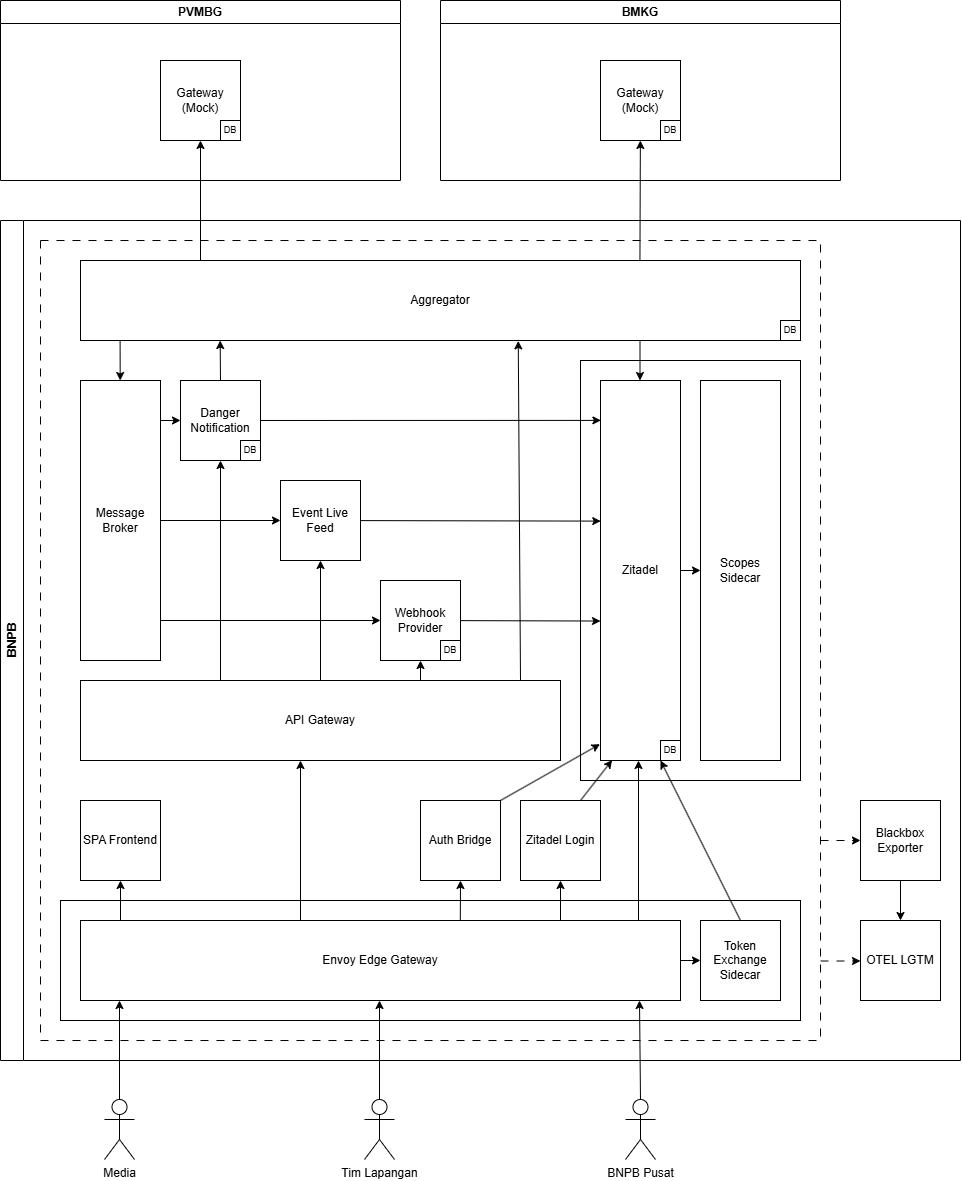
\includegraphics[width=.9\linewidth,height=.72\textheight,keepaspectratio]{architecture}
\caption{Arsitektur container \NamaSistem{}. Panah REST/gRPC mengikuti pemanggil ke penerima; panah dari Message Broker mengikuti aliran publikasi AMQP; panah putus-putus menunjukkan probe dan telemetri.}
\label{fig:architecture}
\end{figure}

\begin{enumerate}
\item Media, Tim Lapangan, dan BNPB Pusat mengakses satu origin melalui Envoy Edge Gateway. Envoy meneruskan \code{/} ke SPA Frontend (Nginx), \code{/auth/*} ke Auth Bridge, halaman login ke Zitadel Login, serta request OIDC ke Zitadel. Tidak ada jalur langsung dari pengguna ke container lain.
\item Untuk setiap request \code{/api/}, Envoy memanggil Token Exchange Sidecar (Rust) melalui \code{ext_authz}. Sidecar menukar access token opaque milik pengguna dengan JWT ke Zitadel (RFC 8693), lalu Envoy meneruskan request beserta JWT tersebut ke API Gateway.
\item API Gateway (Go) menerjemahkan REST/JSON dan SSE menjadi pemanggilan gRPC ke Aggregator, Danger Notification, Event Live Feed, dan Webhook Provider. Pembacaan hazard mengambil canonical store melalui Aggregator, bukan memanggil mock secara sinkron.
\item Aggregator melakukan polling REST/JSON ke kedua mock dengan kredensial berbeda. Tidak ada push langsung dari mock ke BNPB. Hasil normalisasi dan outbox ditulis dalam satu transaksi PostgreSQL; publisher mengirim envelope Protobuf dari outbox ke Message Broker (RabbitMQ).
\item Message Broker membagikan publikasi ke queue tiap consumer. Event Live Feed menyediakan replay dan stream, Webhook Provider mengirim HTTP callback ke endpoint eksternal, dan Danger Notification menyimpan notifikasi serta push outbox sebelum worker mengirim melalui Firebase Cloud Messaging (FCM). Danger Notification juga memanggil Aggregator untuk status kesegaran sumber. Endpoint webhook dan FCM berada di luar sistem sehingga tidak digambarkan.
\item Aggregator, Danger Notification, Event Live Feed, dan Webhook Provider memverifikasi JWT secara mandiri memakai metadata dan kunci publik Zitadel. Role dan scope pada JWT dipasok Zitadel melalui Scopes Sidecar (\code{zitadel-claims}, target Actions v2).
\item Seluruh container di dalam kotak putus-putus mengirim trace, metric, dan log melalui OpenTelemetry ke OTEL LGTM. Blackbox Exporter melakukan probe HTTP/gRPC/TCP ke container tersebut dan hasilnya di-scrape oleh OTEL LGTM.
\end{enumerate}

Kelompok komponen \emph{Auth} pada rancangan awal direalisasikan oleh Zitadel, Zitadel Login, Auth Bridge, Token Exchange Sidecar, dan Scopes Sidecar. Auth Bridge hanya menangani \code{/auth/*} (OIDC dan sesi SQLite terenkripsi); permintaan API bisnis melewati Envoy dan API Gateway. Container sekali jalan \code{auth-bootstrap}, yang menyiapkan proyek, akun, grant, dan client OIDC sebelum layanan lain berjalan, tidak digambarkan karena tidak aktif saat runtime. Observabilitas menggunakan container \code{otel-lgtm} serta \code{blackbox}, bukan container Prometheus dan Jaeger terpisah seperti sketsa awal.

\section{Teknologi dan Alasan Pemilihan}
\begin{longtable}{@{}P{3cm}P{3.6cm}P{8.2cm}@{}}
\toprule \textbf{Komponen} & \textbf{Teknologi} & \textbf{Alasan dan tanggung jawab}\\\midrule\endhead
BMKG dan PVMBG & Python 3.12, HTTP standard library, SQLite & Dependensi ringan; thread request memungkinkan health/admin tetap merespons saat request data menunggu. File database mempertahankan seed dan event setelah restart.\\
Frontend & React, TypeScript, Vite, Nginx & SPA dengan tampilan login, filter/daftar/detail hazard, status sumber, live feed, notifikasi, dan webhook; Nginx menyajikan hasil build statis.\\
Edge dan REST API & Envoy, Rust (Tonic); Go, chi, oapi-codegen & Envoy melakukan routing; sidecar Rust menukar token melalui \code{ext_authz}. Go menjaga bentuk JSON, status HTTP, validasi OpenAPI, dan framing SSE yang berbeda dari ProtoJSON.\\
Aggregator & Go, gRPC, PostgreSQL 17 & Goroutine untuk polling independen; transaksi dan indeks relational untuk data inti, JSONB untuk atribut dinamis.\\
Event Live Feed & Rust, Tokio, Tonic & Stream asinkron dan buffer replay berbatas; API Gateway mengubahnya menjadi SSE untuk browser.\\
Webhook Provider & Go, SQLite WAL & Menyimpan subscription, hasil delivery, dan deduplikasi; worker mengirim HTTP callback bertanda tangan.\\
Danger Notification & C\#, ASP.NET gRPC, EF Core SQLite, Firebase Admin & Menyimpan notifikasi dan push outbox privat, menyediakan proyeksi summary/full, serta mengirim push FCM melalui worker. Status kesegaran sumber dibaca melalui Aggregator.\\
Identitas & Zitadel, PostgreSQL, Node.js 24, Rust & Provider mengelola akun; bridge menjalankan OIDC dan sesi SQLite terenkripsi; Rust Actions memasok role/scope.\\
Distribusi event & RabbitMQ 4, AMQP, Protobuf & Fanout dan queue independen memisahkan produsen dari consumer serta menyediakan acknowledgement.\\
Observabilitas & OpenTelemetry, otel-lgtm, blackbox exporter & Pengiriman trace/metric/log dan probe HTTP/gRPC/TCP; dashboard serta alert diprovisikan melalui berkas repo.\\
Orkestrasi & Docker Compose & Batas proses, jaringan, volume, dan dependensi dinyatakan di satu stack utama; Compose khusus dipakai untuk pengembangan parsial.\\\bottomrule
\end{longtable}

\section{Asumsi dan Konfigurasi}
\begin{enumerate}
\item Instalasi M1 berjalan pada satu host Docker. Port publik default adalah BNPB 8080, BMKG 8081, PVMBG 8082, Grafana 3000, serta RabbitMQ Management 15672. Port mock dalam container adalah 8080.
\item Host \code{localhost} dan \code{auth.localhost} menunjuk mesin demo. HTTP diizinkan secara eksplisit untuk lingkungan lokal; ini bukan konfigurasi TLS produksi.
\item Setiap mock menyiapkan minimal 20 record pada database baru. Interval event default 10 detik; polling contoh 3 detik. Semua nilai latensi konfigurasi merupakan parameter simulasi, bukan hasil benchmark.
\item ID sumber dan timestamp menjadi dasar watermark polling inklusif. Tabel referensi gunung statis merupakan data milik BNPB. Penerimaan field tambahan tidak menjamin kompatibilitas perubahan tipe atau penggantian nama field wajib.
\item Aggregator adalah pemilik logis canonical store untuk operasi bisnis. Layanan lain memakai gRPC atau event; Notification membaca notifikasi dari SQLite miliknya. Collector juga mengakses PostgreSQL untuk metrik. Distribusi environment Compose belum membatasi kredensial database secara eksklusif pada Aggregator; batas isolasi ini dijelaskan pada P4.
\item Akun pengguna di-seed pada Zitadel, bukan SQLite mock ataupun frontend. Tiga akun manusia memiliki role terpisah; service user untuk tes end-to-end memiliki kredensial tersendiri.
\item Notifikasi push memerlukan proyek Firebase dan service-account JSON lokal; konfigurasi web publik diperlukan untuk push browser. Tanpa dependensi tersebut, demo push belum dapat dianggap terbukti.
\item Restart mempertahankan volume bernama. Menghapus volume menghilangkan data persisten. Replay feed berada di memori, dan RabbitMQ belum memiliki mount data persisten eksplisit pada Compose saat ini.
\end{enumerate}

\section{Ringkasan Menjalankan Sistem}
Prasyarat dasar adalah Docker Desktop/Engine yang aktif dan Python 3.12+ untuk helper setup. Siapkan konfigurasi lokal dari contoh; helper mempertahankan secret yang sudah tersedia. Helper mock hanya mengisi dua kredensial sumber, sehingga nilai \code{REPLACE_*} lainnya dalam \code{.env} harus diprovisikan sesuai pemiliknya. Isi kredensial broker dan token internal yang digunakan; sesuaikan DSN database dengan definisi Compose. Sediakan file Firebase pada \code{FIREBASE_CREDENTIALS_PATH}. Nilai privat tidak dicantumkan dalam laporan.

\begin{lstlisting}
python tools/setup_mock_env.py
python tools/setup_auth_env.py
docker compose --env-file .env --env-file .env.auth -f compose.yaml config --quiet
docker compose --env-file .env --env-file .env.auth -f compose.yaml up --build -d --wait
\end{lstlisting}

Perintah terakhir merupakan satu perintah orkestrasi setelah prasyarat konfigurasi dipenuhi. Buka \url{http://localhost:8080}, pilih masuk melalui Zitadel, lalu gunakan akun \code{media-demo}, \code{lapangan-demo}, atau \code{bnpb-demo}. Password berasal dari \code{.env.auth}. Dashboard Compose utama menggunakan \code{VITE_DATA_MODE=gateway}; fixture lokal hanya untuk mode pratinjau/stack Auth terpisah. Login UI milik Zitadel tidak mengubah frontend BNPB menjadi SSR.

Panduan operasional tersedia di \code{README.md}, \code{docs/mock-testing.md}, \code{docs/auth-testing.md}, \code{docs/e2e-testing.md}, dan \code{docs/load-testing.md}. Untuk layanan BNPB yang sudah berkembang, gunakan Compose dan README layanan terbaru bila uraian status pada README root masih tertinggal. Stack parsial \code{compose.mocks.yaml}, \code{compose.auth.yaml}, serta \code{compose.frontend.yaml} tetap berguna untuk pengembangan, tetapi bukan pengganti pengujian integrasi stack utama.

\section{Strategi Verifikasi}
Artefak pengujian tersimpan di \code{docs/tex/evidence/}, meliputi hasil tes mock, tes browser Auth, unit test Aggregator, ringkasan pengujian otomatis, serta JSON k6. Screenshot demonstrasi dikelompokkan pada direktori P1--P5 sesuai problem yang diuji. Path singkat seperti \code{P3/1-new.png} relatif terhadap direktori bukti tersebut; path berawalan \code{evidence/} relatif terhadap \code{docs/tex/}. Nama berkas dan hash setiap artefak tercantum pada \code{docs/tex/evidence/manifest.json}.

Bukti terdiri atas inspeksi implementasi, hasil tes otomatis tersimpan, tangkapan layar demo, dan pengukuran k6. Bab P1--P5 menyajikan hasil aktual beserta rujukan artefaknya. Hasil k6 mencatat beban 50 VU selama 60 detik dan isolasi latensi BMKG; screenshot RabbitMQ memperlihatkan fanout serta penumpukan dan pengurasan backlog consumer. Status PASS pada suite otomatis dilaporkan sebagai hasil suite dengan cakupan assertion yang dijalankan, bukan pengganti setiap observasi manual. Bukti browser Auth historis dibedakan dari pengujian token API terbaru. Gambar yang menampilkan nilai secret konfigurasi tidak direproduksi dalam PDF.
